% J. Musilová a P. Musilová, Matematika I: pro porozumnění i praxi: netradiční
% výklad tradičních témat vysokoškolské matematiky. VUTIUM, 2009, s. 339, isbn:
% 978-80-214-3631-2. WWW: http://localhost/stable.php?id=527
% https://1drv.ms/b/s!Ajq2sO-eH2xU9XEhAGXpHPItEUvR
% https://tex.stackexchange.com/questions/117140
% https://tex.stackexchange.com/questions/123880/

\documentclass[11pt, 
  border={-0.3cm 0cm 0cm 0cm}    % left bottom right top    
]{standalone}
  \usepackage{pgf,tikz,pgfplots}
    \pgfplotsset{compat=1.15}
    \usetikzlibrary{arrows}
    \usetikzlibrary{calc}
    \usetikzlibrary{intersections}
  \usepackage{amsmath, amssymb, amsthm, bm}

\begin{document}
    \definecolor{blue}{rgb}{0,0,1}
    \definecolor{red}{rgb}{0.8,0,0}
    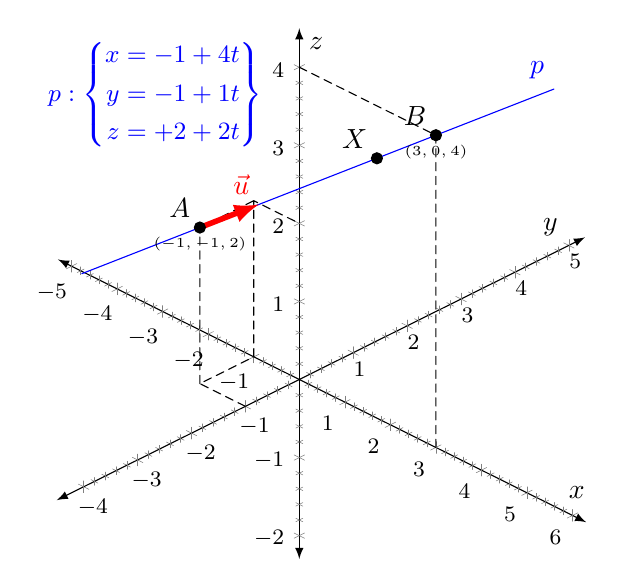
\begin{tikzpicture}[
        line cap=round,line join=round,>=triangle 45,x=1cm,y=1cm
        ]
        \begin{axis}[
                view={45}{35},
                % axis background/.style={fill=gray!5}, 
                axis lines=center,
                width=15cm,height=15cm,
                xtick={-5,-4,...,6},
                ytick={-4,-3,...,5},
                ztick={-2,-1,...,3,4},
                ticklabel style={font=\footnotesize},
                % minor tick={-12,-11,...,12},
                minor tick num=4,
                xmin=-5.1, xmax=6.1,
                ymin=-4.3, ymax=5.1,
                zmin=-2.1, zmax=4.3,
                xlabel={$x$},
                ylabel={$y$},
                zlabel={$z$},
                enlargelimits={abs=0.2}, 
                axis line style={latex-latex}, 
              ]

            % plot dots for the two points
            \addplot3 [only marks] coordinates {(-1,-1,2) (3,0,4) (2,-0.25,3.5)};
            
            % plot dashed lines to axes
            \addplot3 [no marks,densely dashed] coordinates {(0,0,4) (3,0,4) (3,0,0)};
            \addplot3 [no marks,densely dashed] coordinates {(0,-1,0) (-1,-1,0) (-1,0,0)};
            \addplot3 [no marks,densely dashed] coordinates {(-1,0,0) (-1,0,2) (0,0,2)}; 
            \addplot3 [no marks,densely dashed] coordinates {(-1,-1,0) (-1,-1,2) (-1,0,2)};
            
            % plot main line
            % x= -1 + t*4, 
            % y= -1 + t*1,
            % z=  2 + t*2,
            \addplot3 [no marks, color=blue] coordinates {(-3,-1.5,1) (5,0.5,5)};
            \addplot3 [-latex, color=red, line width=2pt] coordinates {(-1,-1,2) (0,-0.75,2.5)};

            % label points
            \node [above left] at (axis cs:-1,-1,2) {$A$};
            \node [below] at (axis cs:-1,-1,2) {\tiny$(-1,-1,2)$};
            \node [above left] at (axis cs:3,0,4) {$B$};
            \node [below] at (axis cs:3,0,4) {\tiny$(3,0,4)$};
            \node [above left] at (axis cs:2,-0.25,3.5) {$X$};
            \node [above left, red] at (axis cs:0,-0.75,2.5) {$\vec{u}$};
            \node [above left, blue] at (axis cs:5,0.5,5) {$p$};

            \node [above left, blue] at (axis cs:0,-0.5,3) 
                {\small $      
                  p : \left\{
                        \begin{aligned}
                            x &= -1 + 4t        \\
                            y &= -1 + 1t        \\
                            z &= +2 + 2t
                        \end{aligned}
                      \right\} 
                $};
        \end{axis}
    \end{tikzpicture}
\end{document}